\chapter{Machine Learning y Redes Neuronales}

En este capítulo trataremos los principales conocimientos de Aprendizaje automático como su clasificación y su importante dentro del campo de la inteligencia artificial, además exploraremos algunos modelos importantes. 
En este seminario se dará énfasis en los algoritmos de clasificación. Luego nos enfocaremos en las redes neuronales para tratar más a fondo los problemas de clasificación.

\section{Aprendizaje Automático}
Machine Learning o aprendizaje automático es una rama de la inteligencia artificial que empezó a cobrar cobrar importancia en los años 80's, en esta rama se diseñan sistemas que aprenden a identificar patrones en un conjunto de datos. A medida que se realice este aprendizaje la máquina podrá ser capaz de realizar una predicción o tomar decisiones sin haber estado programada explícitamente para realizar esta tarea.


El aprendizaje automático se puede clasificar en 3 tipos: Supervizado, No supervisado, Aprendizaje con refuerzo.\cite{WEBSITE:2}
\subsection{Aprendizaje Supervizado}
Este tipo de aprendizaje  toma un conjuto de datos etiquetados, es decir datos cuyos resultados o clases son conocidos estos datos serán usados como entrada al sistema. Primero se entrena el modelo con los datos de entrada y luego se trata de predecir  una salida de acuerdo a sus etiquetas.

 \textquotedblleft El aprendizaje supervisado trata de modelar la relación entre el resultado de la predicción y las características de las entradas de manera que se puede predecir nuevos valores para un nuevo conjunto de datos \textquotedblright \cite{WEBSITE:1}
\subsection*{Tipos de problemas}
Dentro del aprendizaje supervisado podemos dividir los problemas en 2 tipos:
\subsubsection*{Problemas de Regresión Lineal}
Los problemas de regresión lineal son muy conocidos en el ámbito de aprendizaje automático y la estadística 
\subsubsection*{Problemas de Clasificación}
\textquotedblleft En este tipo de problemas se predice una respuesta del tipo categórica de manera que se puedan separar los datos mediante clases. \textquotedblright \cite{WEBSITE:2}

\textquotedblleft El objetivo de los problemas de clasificación es asignar las observaciones en categorías discretas en lugar de estimar valores continuos. \textquotedblright \cite{WEBSITE:1}


\begin{figure}[H]
	\centering
	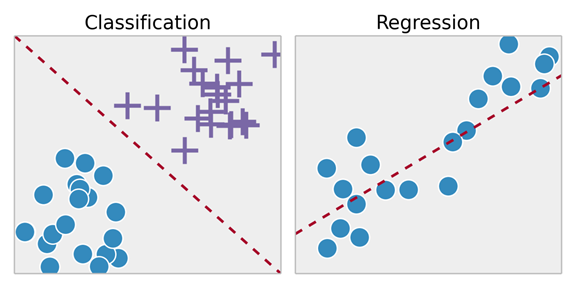
\includegraphics[width=0.9\textwidth]{Figures/regreclas.png}
	\caption{Regresión y clasificación \\ Fuente:  \href{https://medium.com/deep-math-machine-learning-ai/different-types-of-machine-learning-and-their-types-34760b9128a2}{\textit{https://medium.com/}}}
	\label{Regresion}
\end{figure} 

\subsubsection*{Algoritmos de Aprendizaje Supervizado}
\subsubsection*{Regresión Lineal}
\textquotedblleft El algoritmo de regresión lineal asume que existe una relación entre las variables de entrada $x=(x_{1},...,x_{n})$ y una salida simple $y$.  Cuando se tiene solo una variable simple $x$ el método se conoce como simple linear regression y cuando se tienen múltiples entradas se le conoce como multiple linear regression.  \textquotedblright \cite{WEBSITE:3} .Es comúnmente usado para estimar valores reales en base a variables continuas. La figura 3.2 muestra una regresión lineal simple.
\begin{equation}
\label{Simple learning regression}
y=b_{0}+b_{1}*x_{1}+b_{2}*x_{2}+.....+b_{n}*x_{n}
\end{equation} 
En esta ecuación:
\begin{itemize}
	\item $y$    : Variable dependiente
	\item $x_{i}$: Variable independiente i
	\item $b_{0}$: Intercepción
	\item $b_{1}$: Coeficiente para la primera característica
	\item $b_{n}$: Coeficiente para la primera característica
	
\end{itemize}
El objetivo del algoritmo de regresión lineal es obtener valores adecuados para $b_{0}$ y $b_{1}$ de manera que se reduzca la siguiente función de costo.
 \begin{equation}
 \label{eq:T3}
 \begin{aligned}
 J&=\frac{1}{n} \sum_{i=1}^{n}(pred_{i}-y_{i})^2
 \end{aligned}
 \end{equation}


\begin{itemize}
	\item $pred_{i}$: predicción de la i-esima variable
	\item $y_{i}$   : Valor real asociado a la i-esima variable
	\item $n$       : Número de datos para el entrenamiento
	
\end{itemize}
Un método muy importante es la gradiente de descenso que se usa para actualizar los valores de los $b_{i}$ de manera que se reduzca la función de costo $J$ de la ecuación 3.2.
\begin{figure}[H]
	\centering
	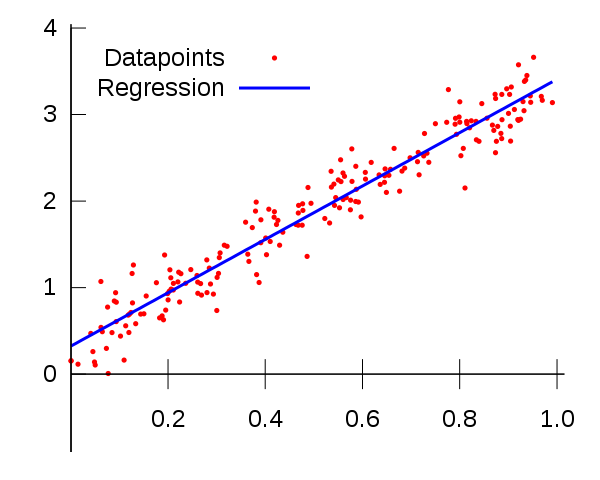
\includegraphics[width=0.9\textwidth]{Figures/Linear.png}
	\caption{Regresión Lineal \\ Fuente:  \href{https://www.forexmt4indicators.com/linear-regression-mt4-indicator/}{\textit{www.forexmt4indicators.com/}}}
	\label{Regresión Lineal}
\end{figure} 

\subsubsection*{Regresión Logística}
A diferencia de la regresión Lineal, la regresión Logística es usado para precedir el resultado de un variable de tipo categórica es decir variables que pueden ser describen por un número finito de categorías.

 La regresión Logística es usado para problemas de clasificación lo hace mediante la predicción de que una salida $Y$ sea dicotoma es decir que solo tenga 2 posibles valores.
 la regresión produce una curva la cual produce valores entre 0 y 1.
 \textquotedblleft Matemáticamente podemos como que las salidas están modeladas como una combinación de los predictores lineales.\textquotedblright \cite{WEBSITE:6}
 \begin{equation}
 \label{eq:t}
 \begin{aligned}
 odds &= p/ (1-p)\\ 
 ln(odds) &= ln(p/(1-p))\\      
 logit(p) &= ln(p/(1-p)) = b_{0}+b_{1}X_{1}+b_{2}X_{2}+b_{3}X_{3}....+b_{k}X_{k}
 \end{aligned}
 \end{equation}
 %\end{equation} 
 
 \begin{itemize}
 	\item p : probabilidad de presencia de una característica de interés.
 	\item odds: probabilidad de éxito.
 	\item logit: función logit
 \end{itemize}
 
 Despejando p de las ecuaciones anteriores de 3.2 podemos obtener que:
  \begin{equation}
  \label{eq:t1}
  \begin{aligned}
  p&=\frac{1}{1+e^{b_{0}+b_{1}X_{1}+b_{2}X_{2}+b_{3}X_{3}....+b_{k}X_{k}}} \\
  Y_{pre}&=\frac{1}{1+e^{f(X)}}
  \end{aligned}
  \end{equation}
 En la ecuación 3.3, $Y$ define la función logística que se muestra en la figura 3.3. Esta forma también se puede conocer como la función sigmoidal en el perceptron.
 El algoritmo usa SGD para hallar los valores adecuados de $b_{i}$ de manera que el $erro=Y_{pre}- Y$ sea mínimo.
 El valor de la predicción es 1 si $Y_{pred}>0.5$ y 0 en caso contrario. De esta forma se determina el objeto con características $X$ si pertenece o no a una clase.
 
 \begin{figure}[H]
 	\centering
 	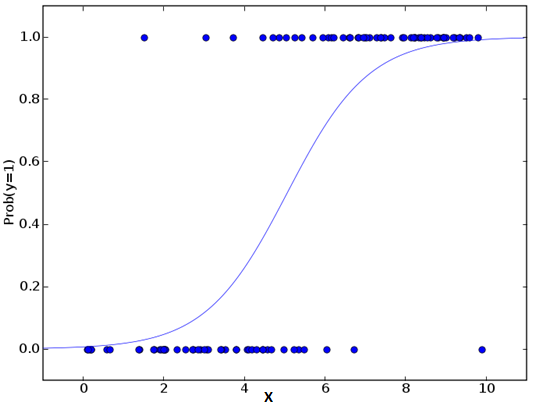
\includegraphics[width=0.9\textwidth]{Figures/logistic.png}
 	\caption{Regresión Logística \\ Fuente:  \href{https://www.analyticsvidhya.com/blog/2017/09/common-machine-learning-algorithms/}{\textit{www.analyticsvidhya.com}}}
 	\label{Regresión Logistica}
 \end{figure} 
\subsubsection*{Nearest Neighbor}
Es un algoritmo de clasificación que almacena los conjuntos de entrenamiento de manera que dado un nuevo ejemplo $x$ lo clasifica buscando la distancia  más cercana a un ejemplo de entrenamiento $(x_{i},y_{i})$ de manera que identifica la clase $y=y_{i}$ a la que corresponde.

 Comúnmente se usa el algoritmo k-nn para clasificar una entrada $x$ en los k más cercanos conjuntos de entrenamiento y asigna el objeto a la clase de más frecuencia.

  \begin{equation}
  \label{eq:t12}
  \begin{aligned}
  x^i=(x_{1}^i,x_{2}^i,.... ,x_{n}^i)\\
  d_{E}(x^i,x^j)
  \end{aligned}
  \end{equation}
\begin{itemize}
	\item $x^i$: objeto con n características.
	
\end{itemize}

Definimos $d_{E}$ como la función distancia entre los vectores  $x_{i}$ y $y_{i}$ están función distancia pueden una de las siguientes clasificaciones:

  \begin{itemize}

  \item distancia euclideana:    $(\sum_{i=1}^{k}(x_{i} - y_{i})^2)^\frac{1}{2}$
  \item distancia Manhattan:     $\sum_{i=1}^{k}|x_{i} - y_{i})|  $
  \item distancia Minkowski:     $(\sum_{i=1}^{k}(|x_{i} - y_{i}|)^p)\frac{1}{p}$
  \end{itemize}
Los 3 definiciones anteriores de distancia son usadas para variables continuas.  Para el caso de variables categóricas debería usarse la distancia de Hamming cuya definición se muestra en la ecuación 3.6


  \begin{equation}
  \label{eq:t6}
  \begin{aligned}
  	D_{H}&=\sum_{i=1}^{k}|x_{i} - y_{i})|\\
  	x&=y \Longrightarrow D=0\\
  	x&\neq y \Longrightarrow D=1
  \end{aligned}
  \end{equation}
  	
\textquotedblleft La elección de un valor óptimo de k se logra mejor por la inspección de los datos. En general un valor grande de k es más preciso ya que reduce el ruido pero no hay garantías de que sea un valor correcto, una mejor manera de calcular el valor de $k$ es mediante el uso de la validación cruzada.
\textquotedblright \cite{WEBSITE:7}

En la figurar 3.4 muestra el algoritmo de k-nn dado un nuevo ejemplo(círculo verde) este será clasificado a de acuerdo seleccionado. Para $k=1$ el nuevo ejemplo será clasificado en la clase 1 y $k=3$ será clasificado en la clase 2.
 \begin{figure}[H]
 	\centering
 	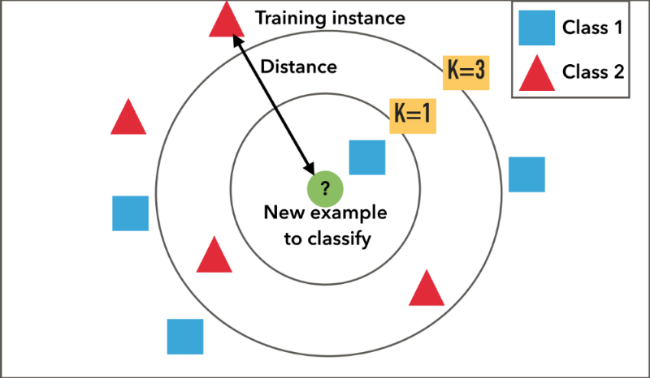
\includegraphics[width=0.7\textwidth]{Figures/knn.png}
 	\caption{knn \\ Fuente:  \href{https://medium.com/@adi.bronshtein/a-quick-introduction-to-k-nearest-neighbors-algorithm-62214cea29c7}{\textit{www.medium.com/}}}
 	\label{knn}
 \end{figure} 
\subsubsection*{Máquinas de soporte Vectorial(SVM)}
Las Maquinas de soporte vectorial fueron creadas por Vladimir Vapnik y constituyen un método para realizar tareas de clasificación y regresión.\\ Las SVM usan el concepto de planos de decisión. Un plano de decisión separa un conjunto de objetos que tienes diferentes etiquetas de clases. Las SVM no están restringidas a los problemas lineales debido a las \textit{funciones Kernel.}
\textbf{Funciones Kernels}\\
Las SVM pueden tener distintos tipos de kernels que tienen como objetivo tomar la data y transforma una forma requerida algunas de estas funciones son:
\begin{itemize}
	\item Lineal: $\ker(x_{i},x_{j})= x_{i} \cdot x_{j}$
	\item Polinomial: $\ker(x_{i},x_{j})= ( \gamma x_{i} \cdot x_{j}+C)^d$
	\item Radial: $\ker(x_{i},x_{j})= e^{(\gamma |x_{i} - x_{j}|)}$
	\item Sigmoidal: $\ker(x_{i},x_{j})= \tanh ( \gamma x_{i} \cdot x_{j}+C)$
\end{itemize}
En la figura 3.5 muestra el efecto de las funciones kernels en un conjunto de datos para que este sea linealmente separable sin necesidad de construir curvas complejas.\\
\begin{figure}[H]
	\centering
	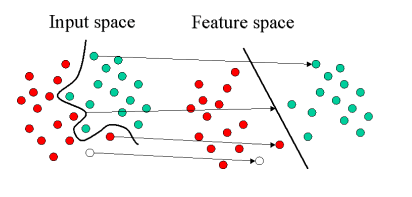
\includegraphics[width=0.9\textwidth]{Figures/kernel.png}
	\caption{transformación con la función kernel \\ Fuente:  \href{http://www.statsoft.com/Textbook/Support-Vector-Machines}{\textit{www.statsoft.com}}}
	\label{transformación con la función kernel}
\end{figure} 

Podemos dividir SVM en 2 categoríasas:\\
\textbf{Super Vector Classificacion}\\
Los SVC realizan la tarea de clasificación encontrando un hiperplano que maximeze el margen entre 2 clases.Los vectores que definen el hiperplano son llamados \textit{support vector}.\\ Para la clasificación es necesaria mapear los datos a un espacio de características de mayor dimensión donde resulte más fácil la separación lineal.  La imagen de la Figura 3.5 muestra de manera gráfica que cambio de espacio nos permite separar clases de manera más sencilla.\\ \\
\textbf{Super Vector Regression}\\
La idea de SVR trata de mapear los datos de entrenamiento $x \in X$ , a un espacio de mayor dimensión mediante una mapeo no lineal $ \varphi : X \to F$ .\\
Las SVR son parecidas a las máquinas de soporte Vectorial para la clasificación pero con la diferencia de que la salida es un número real que es difícil de predecir con la información que se posee además de que tiene infinitas posibilidades. Para los problemas de regresión se usan los kernels Radial y polinomial. La figura 3.6 muestra un ejemplo de problema de regresión para un caso no lineal, mediante la mapeo $ \varphi $ se cambia el espacio.

\begin{itemize}
	\item caso lineal:     $y=\sum_{i=1}^{N}(\alpha_{i}  -\alpha_{i}^*)\langle x_{i},x\rangle +b$
	\item caso no lineal:  $ y=\sum_{i=1}^{N}(\alpha_{i}  -\alpha_{i}^*)\ker(x_{i},x) +b$
\end{itemize}

\begin{figure}[H]
	\centering
	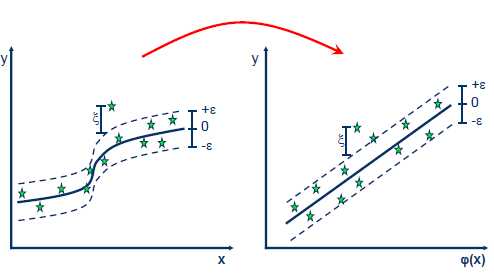
\includegraphics[width=0.7\textwidth]{Figures/SVR.png}
	\caption{transformación para un problema de regresión \\ Fuente:  \href{http://www.saedsayad.com/support_vector_machine_reg.htm}{\textit{www.saedsayad.com}}}
	\label{transformacion}
\end{figure} 

\subsubsection*{Naive Bayes}
Esta basado en el teorema de bayes donde se asume la independencia entre los predictores.
Es una técnica de clasificación basada en el teorema de bayes suponiendo que las características de una clase no esta relacionada con otra característica un ejemplo de esto es \textquotedblleft una fruta puede considerarse una manzana si es roja, redonda y de aproximadamente 3 pulgadas de diámetro. Incluso si estas características dependen unas de otras o de la existencia de otras características, todas estas propiedades contribuyen de forma independiente a la probabilidad de que esta fruta sea una manzana y es por eso que se la conoce como \textbf{naives}  \textquotedblright \cite{WEBSITE:4}
\subsubsection*{Decision Trees}
El árbol de decisión construye un modelo basado en los actuales valores de los datos. La decisiones se difurcan en la estructura de árbol hasta que se toma una decisión de predicción para un registro dado. Los arboles de decisión están entrenada para problemas de clasificación y regresión . Una de las principales ventajas de los arboles de decisión es que son rápidos y precisos.
\subsubsection*{Neural Networks}
Los modelos de redes neuronales fue inspirado de las redes neuronales biológicas y realizan tareas complejas como reconocimiento de imágenes
El tema de Neural Network será tratado con más detenimiento en el capítulo 4.
\subsection{Aprendizaje No Supervizado}
Mientras que el aprendizaje supervizado aprende  de un conjunto de datos de entrenamiento con respuestas o etiquetas correctas. En el aprendizaje no supervizado los datos de entrenamiento no poseen ninguno tipo de etiqueta, el sistema debe de interpretar los datos por si mismo.
El aprendizaje no supervizado es usado principalmente para el reconocimiento de patrones y modelado descriptivo.
\subsubsection*{Clustering}
Clustering se refiere a agrupar objetos con características similares es decir se busca la relación entre ellos sin necesidad de que exista un conocimiento a priori de esos grupos.
\begin{figure}[H]
	\centering
	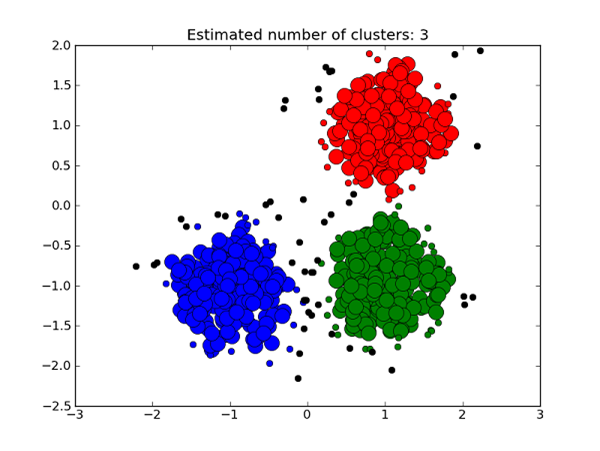
\includegraphics[width=0.9\textwidth]{Figures/clustering.png}
	\caption{Clustering \\ Fuente:  \href{https://medium.com/deep-math-machine-learning-ai/different-types-of-machine-learning-and-their-types-34760b9128a2}{\textit{https://medium.com/}}}
	\label{Clustering}
\end{figure} 
\subsubsection*{K-means Clustering}
el algoritmo
\subsection{Aprendizaje por refuerzo}
Este tipo de aprendizaje fue inspirado por la psicología conductista, este tipo busca determinar que tipo de acciones tomar en un entorno dado. \textquotedblleft El objetivo del método es recopilar la interacción con el entorno para tomar acciones que maximicen el beneficio o minimicen el riesgo. \textquotedblright \cite{WEBSITE:1}
\begin{figure}[H]
	\centering
	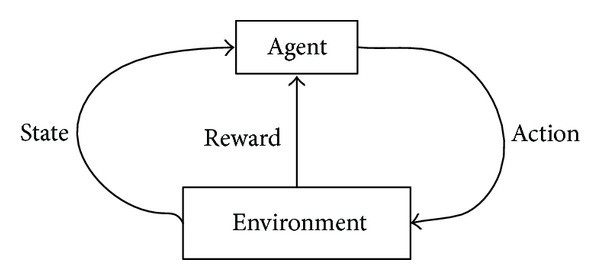
\includegraphics[width=0.9\textwidth]{Figures/esquema.jpeg}
	\caption{Esquema de aprendizaje por refuerzo \\ Fuente:  \href{https://towardsdatascience.com/types-of-machine-learning-algorithms-you-should-know-953a08248861}{\textit{https://towardsdatascience.com}}}
	\label{refuerzo}
\end{figure} 


\section{Redes Neuronales}
\subsection*{Neuronas}
En la biología la neurona es conocida como la unidad fundamental del cerebro humano, el cual está compuesto por millones de neuronas interconectadas entre si. El trabajo de las neuronas consiste en recibir información, procesarla y enviarla a otras células. Este modelo fue copiado en 1943 por Warren S. McCulloch y Walter H. Pitts. Analogamente con las neuronas del cerebro humano nuestra neuro artificial toma una cantidad n de entradas $x_{1}, x_{2}, x_{3}, .. , x_{n}$ estas entradas serán multiplicadas por pesos $w_{1}, w_{2}, w_{3}, .. , w_{n}$ además se puede añadir una constante que llamaremos bias. 

La entrada a de la neurona será la suma total de los productos z=  $\sum_{i=1}^{n}x_{i}$ , el valor de z será la entrada a la neurona la cual la evaluará con una función f de tal forma que nuestra salida sea $y=f(z)$. Otra forma de ver esta expresión es por medio de la notación de vectores donde representaremos a las entradas como $x= [x_{1}  x_{2}  x_{3}  ...  x_{n}]$ y los pesos w= $[w_{1}  w_{2}  w_{3}  ...  w_{n}]$ de esta manera la salida de la neurona estará dada por $y=f(x\cdot w+b)$ donde b representa las bias. 

\subsection*{Redes Neuronales Artificiales}
Las redes neuronales artificiales(ANN)toman de ejemplo la arquitectura del cerebro como inspiración para la construcción de sistemas inteligente. Actualmente son la base para el desarrollo de la inteligencia artificial. Las redes neuronales están constituidas de las uniones de las neuronas. 
\subsection*{Redes Neuronales Profundas}


Las redes neuronales profundas estan constituidas principalmente de un numero de capas de convolución, No linearalidad y pooling.
\begin{itemize}
	\item Convolución:
	Un proceso importante dentro de las redes neuronales es la convolución que es usada para detectar las características de una imagen estas características pueden ser bordes, curvas, etc.
	\item No linearalidad:
	Debido a que las convoluciones son operaciones lineales, lo cual no es adecuado para las tareas del mundo real. Debido a esto es importante introducir el ReLu que aplicará funciones no lineales a los mapas de característica producidas en las capas de convolución.
	Una de las funciones las común es ReLu.
	\begin{figure}[H]
		\centering
		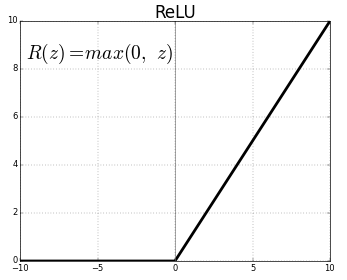
\includegraphics[width=0.5\textwidth]{Figures/relu.png}
		\caption{ReLu  Fuente:
			\href{https://medium.com/@kanchansarkar/relu-not-a-differentiable-function-why-used-in-gradient-based-optimization-7fef3a4cecec}{\textit{https://medium.com/}}
			 }
		\label{ReLu}
	\end{figure}

	
	\item Pooling:
	Sirve para transformar el mapa de características en una representación de menor dimensión con el objetivo de la red sea más invariante a pequeñas transformaciones o variación de la imagen de entrada.
\end{itemize}



%%\subsubsection*{Características}
%%%
%%\begin{figure}[H]
%%\centering
%%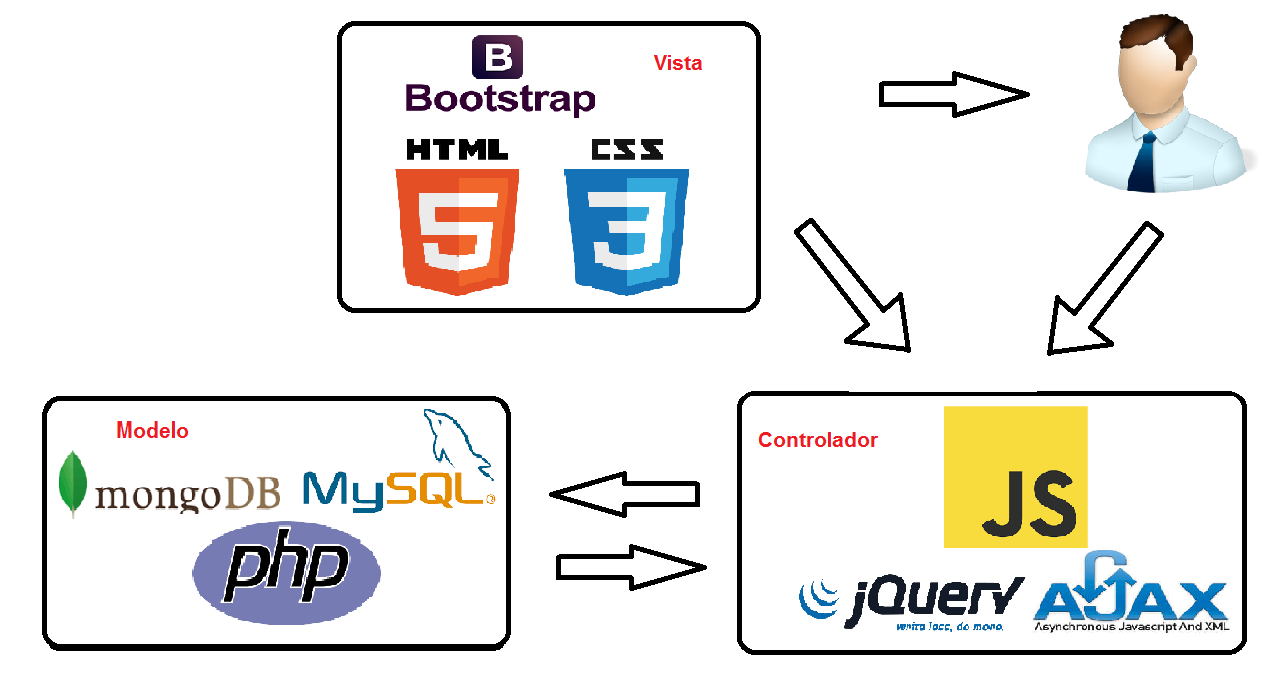
\includegraphics[width=0.9\textwidth]{Figures/mvc.png}
%%\caption{Modelo-Vista-Conrolador}
%%\label{MVC}
%%\end{figure}



\afterpage{\blankpage}